\documentclass[useAMS,usenatbib]{mn2e}
\usepackage{graphicx}
\usepackage{setspace}
\usepackage{float}

\usepackage[
labelfont=sf,
hypcap=false,
format=hang,
width=.9\columnwidth
]{caption}

%\graphicspath{ {images/} }



\title[Redshift Analysis]{Redshift Analysis of H$\alpha$ Emission in Starburst Galaxy M82}

\author[L. Gan]{Litawn Gan}
\begin{document}



\pagerange{\pageref{firstpage}--\pageref{lastpage}} \pubyear{2016}

\maketitle

\label{firstpage}

\Large
\begin{abstract}
\Large
Starburst galaxies are characterized by exceptionally high rates of star formation, indicating significant H II regions and abundance of H$\alpha$ emission lines. We use H$\alpha$ emission lines to analyze the differential redshift at various radial distances of the starburst galaxy Messier 82. We discuss the methodology and errors behind the measurement, especially the limitations imposed by the Stanford Student Observatory. We summarize the historical literature on M82 and analyze the implications of our result.
\end{abstract}
\Large
\begin{keywords}
\Large
H$\alpha$ emission, redshift, spectroscopy, Messier 82
\end{keywords}


\clearpage
\renewcommand{\baselinestretch}{2}
\normalsize
\setlength{\parindent}{0ex}
\section*{Introduction}

Spectroscopic redshift analysis is one of the most productive avenues for astrophysics research today. Galaxy rotation curves, the expansion rate of the universe, and the elemental composition of the universe can all be investigated with redshift analysis. The versatility and power of this technique is especially useful for exploring the properties of starburst galaxies. With the equipment provided at the Stanford Student Observatory, we comment on the feasibility of and associated errors with analyzing galaxy rotation curves with redshift analysis.

\section*{Preliminary Considerations}
\subsection*{Spectroscopy Methods}
The 24 in telescope's spectroscopy module was the primary apparatus in our observations at the Student Observatory. Our initial proposal was to analyze differential redshift parallel to the minor axis of the galaxy; however, there was an inherent drift in the telescope due to limitations in tracking software. The drift was estimated to be at a rate of ~10 arcminutes per minute. While this affects both measurements along the minor and major axes of the galaxy, it is particularly problematic for measurements along the minor axis, as small shifts can transport the line from one side of the galaxy to the other quickly. With this in mind, we chose to take spectra along the major axis of the galaxy. This method allows analysis of both sides of the galaxy in one exposure.

	We chose to focus on the emission line H$\alpha$ for this experiment because of its abundance in H II regions commonly found in spiral galaxies. The wavelength of H$\alpha$ is 656.3 nanometers, and we chose a Neon lamp to calibrate our data. Our strategy to determine galaxy rotation curve revolved around the software suite IRAF (Image Reduction and Analysis Facility), which facilitated spectroscopy reduction and analysis.
\subsection*{Target Galaxy Choice}

	With the limitations of the spectroscopy module at the Student Observatory, appropriate target choice was critical. Criteria for target choice was multidimensional. First and most important: a reasonable angular size small enough such that the entire galaxy could fit on the CCD (charged coupled device), but large enough that more precise radial distance measurements could be obtained. The scope of the 24 inch telescope decided this constraint, 12' x 12' (1024 x 1024 pixels with 0.7 arcseconds each). We identified four suitable targets: Messier 66, 81, 82, and 104.

	The angular size is related with another important criterion, surface brightness. Exact values for surface brightness are difficult to find; however, accurate apparent dimension and magnitude are available. From this data, surface brightness can be estimated by modeling galaxies as ellipses.
    
\begin{tabular}{llll}
\textbf{Object} & \textbf{Mag} & \textbf{Size} & \textbf{Surface Mag} \\
M66    & 8.9                & 9.1' x 4.2'   & 12.6               \\
M81    & 6.94               & 26.9' x 14.1' & 13.1               \\
M82    & 8.41               & 11.2' x 4.3'  & 12.4               \\
M104   & 8.98               & 8.7' x 3.5'   & 12.4       
\end{tabular}
\captionof{table}{Surface Brightness comparison of the four galaxy candidates, calculated with the equation  $S = m + 2.5\cdot \log_{10} A$ with area obtained by modeling each galaxy as an ellipse. }

\vspace{5mm}

 	In general, a high surface brightness is desired; at the rate the CCD saturates, only extremely bright objects would be at risk of saturating. For example, a 120 minute exposure of Messier 82 resulted in an absolute maximum of about 5000 counts, far below the saturation maximum. Without an upper limit on brightness, the higher signal-to-noise ratio of brighter galaxies make them superior targets compared to dimmer galaxies.
    
    	The last criterion relevant to the project is the prevalence of H II regions in the galaxy. These regions of ionized interstellar hydrogen have a dominant spectral line at H$\alpha$, our line of choice. The more H II regions, the stronger the H$\alpha$ line and the more robust our potential signal-to-noise ratio. Unlike surface brightness and angular size, H II prevalence is harder to quantify; it is associated with spiral galaxies and star formation.\par
    
  Quantitative parameter measurements helped with identifying potential candidates, but ranking the galaxies could only come from experience. For example, our initial preferred target Messier 66 proved problematic in our first observation; the signal-to-noise ratio was too low and distilling redshift data was impossible. This initial failure spurred us to switch our target. 

We compared different candidates by taking actual exposures. This method was more fruitful. While approximating factors like surface brightness and H II regions are important, they are not always relevant to our goals. Brightness may not be uniform, i.e. it does not guarantee strong H$\alpha$ lines in regions near the center, where we expect the most redshift. Similarly, a theoretical argument for the prevalence of H II regions does not guarantee that these H II regions and their emission lines are visible from the Earth. Having actual data for quality assessment was essential for determining the best target.

\vspace{15mm}

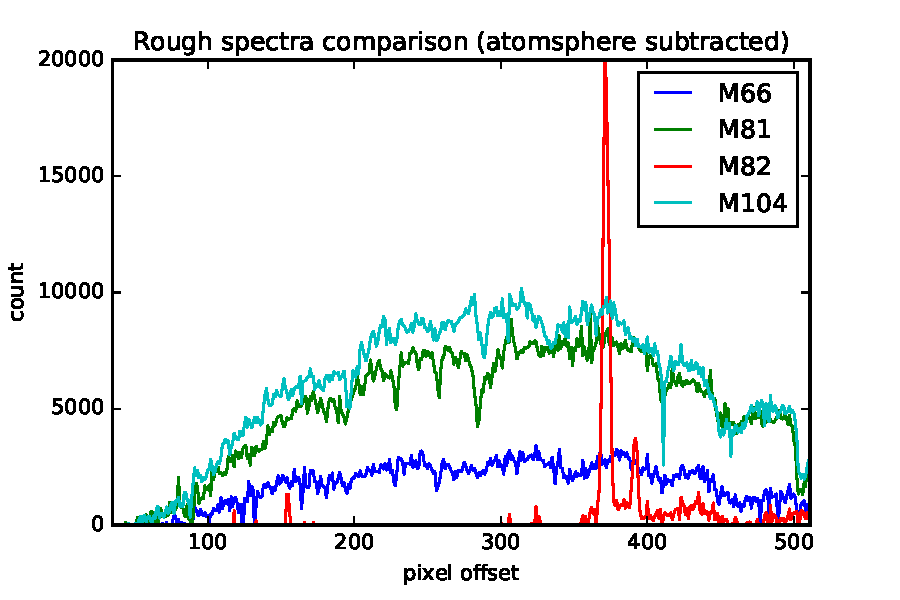
\includegraphics[width=\linewidth]{comparison-atmosphere-subtracted.pdf}
\captionof{figure}{Comparison of our four potential candidates with atmosphere subtracted. Note M66's very low signal-to-noise ratio. Also M82's H$\alpha$ peak shows promise.}

    
\subsection*{Galaxy Target Choice}

Our target audition process identified Messier 82 as an ideal candidate for redshift analysis. Located 12 million light years away in the constellation Ursa Major, Messier 82 has a right ascension of 9$^{h}$ 55$^{m }$ 52.2$^{s}$ and a declination of 69$^{\circ}$ 40' 47''. Our chosen calibration star nearby is HR 4554, known as Gamma Ursae Majoris, with an apparent magnitude of 2.44. M82 is a starburst galaxy with a high rate of star formation and thus the large H II regions associated with stellar nurseries. M82's abundance of H II regions make it a prime target for our spectral analyses around the H$\alpha$ line. The starburst phenomenon is rare in galaxies, and is theorized to have arisen in M82 after gravitational interactions with nearby galaxy Messier 81.

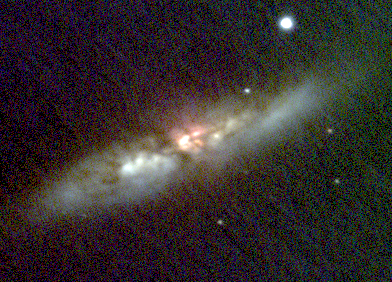
\includegraphics[width=200pt]{M82-color-image-cropped.png}
\captionof{figure}{A combined color image of M82, taken from the 16in telescope.}

\section*{Observation and Method}

\subsection*{Observations}

After the scouting observation night on May 25th, we had two nights to acquire data on M82: May 26th and 27th. The weather was fair on both nights, and we ended up taking a 60 minute exposure on the 26th and a 120 minute exposure on the 27th. Telescope drift was significant; we mitigated this systematic error by shifting the telescope back to its original position at intervals. This error is difficult to quantify because of the random nature of the shifting, but impossible to dispose of.
\vspace{5mm}

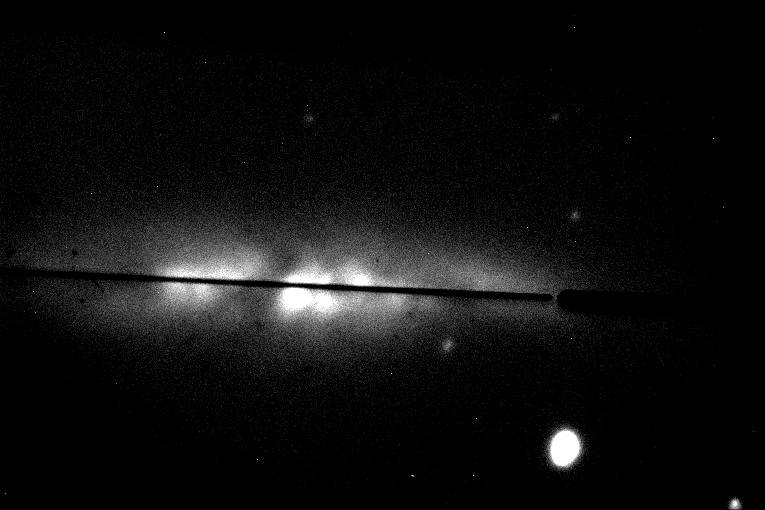
\includegraphics[width=\linewidth]{M82-guiding-cam.jpg}
\captionof{figure}{Photo of M82 on guiding camera, taken on May 27th with the 24in telescope. M82's major axis covers the extent of the CCD.}


\subsection*{Calibration Issues}
We took flats, darks, and biases in our observations with the intention to follow standard data reduction procedure. An anomaly in the lower left half of our CCD inhibited our calibration however. The flats and darks did not incorporate this source of noise -- the bottom left region in both types of calibration frames had only slight differences. We theorized that the buildup was a dark current artifact, as the signal would accumulate with increasing exposure time. The discrepancy could arise from the CCD's different response to dark current in different regions. Our strategy to account for this was to approximate the shape of the dark current with our data and calibrate with this new adjusted dark current.

\vspace{15mm}
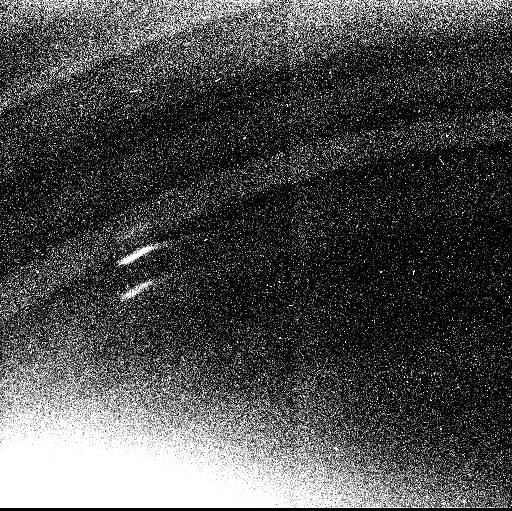
\includegraphics[width=\linewidth]{M82-60min.jpg}
\captionof{figure}{The bottom corner left corner rivals the actual H$\alpha$ line in the galaxy in brightness. There was no reason to expect temperature fluctuations -- CCD sensitivity is the main suspect. }

Unfortunately, a linear model of dark current is only an approximation, and the adjusted calibrations were not noticeably better than their predecessors. Since we had no means to analyze a non-linear dark current accumulation, this step of the calibration was not fulfilled. Our proposed analyses relied on the integrity of data in narrow apertures, so neglecting dark current was not significant.


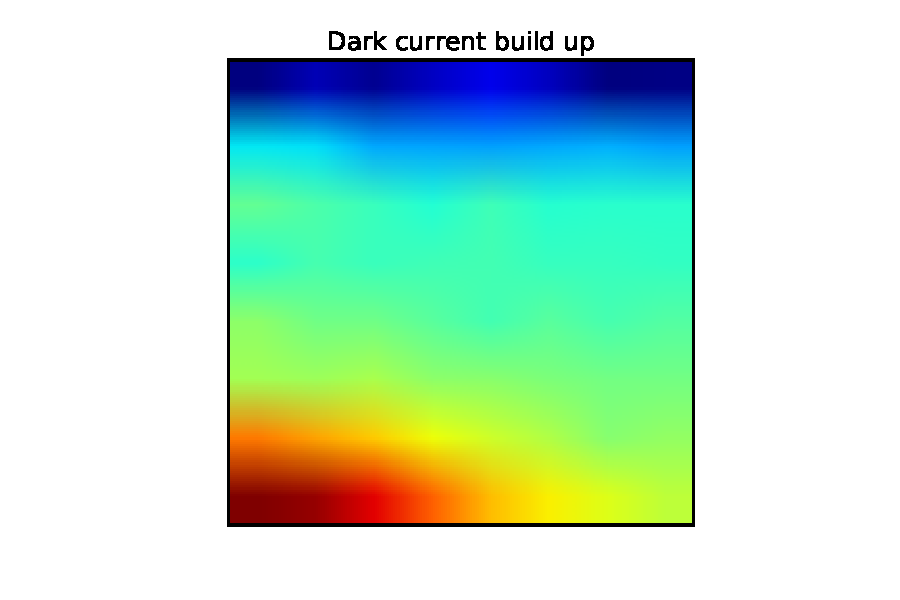
\includegraphics[width=\linewidth]{dark-current-buildup.pdf}
\captionof{figure}{A composite dark current image compiled from 450 second darks. There is a rapid accumulation of noise in the bottom corner, indicated by the red color. }



\subsection*{IRAF Analysis}

IRAF was critical in translating raw spectra into usable data. We used apertures and the Neon calibration lamp to locate specific lines in the galaxy and calibration star. Wavelength axes, scaling, and signal strength as a function of wavelength were determined with IRAF.\par

To determine the redshift at different points of the galaxy, we analyzed the amount of angstroms the H$\alpha$ peak shifted over time. This peak shifting can be interpreted as a velocity value, shedding insight on the structure of the galaxy's rotation curve. The equation governing this transition is: $\bigtriangleup\lambda / \lambda = v / c $. 

	To account for radial distance, 13 IRAF apertures were defined for the 120 minute observation and 10 apertures for the 60 minute one. These apertures spanned 5 pixels on the CCD, capturing the central portions of the galaxy.

	The redshift calculation was done by locating the maximum of the H$\alpha$ peaks, and then analyzing the deviation from H$\alpha$'s known wavelength value. The continuum was impossible to quantify because of the dark current's unpredictable effect. Two plot sets were created for each observation, one with a 300 $\Omega$ range and one with a 50 $\Omega$ range. The larger range graphs correspond to the 60 minute observation below. The more focused graphs are the 120 minute observations. Both plot sets are useful for analyzing the general redshift trend throughout the galaxy.

\section*{Results}

Our results from IRAF came in the form of text files with calibrated spectra. The data was graphed and redshifts calculated.

\subsection*{60 Minute Exposure}
The 60 minute exposures for M82 were taken on May 26th. The graphs show the entirety of the range at the lowest resolution (effectively 300 angstroms across). 

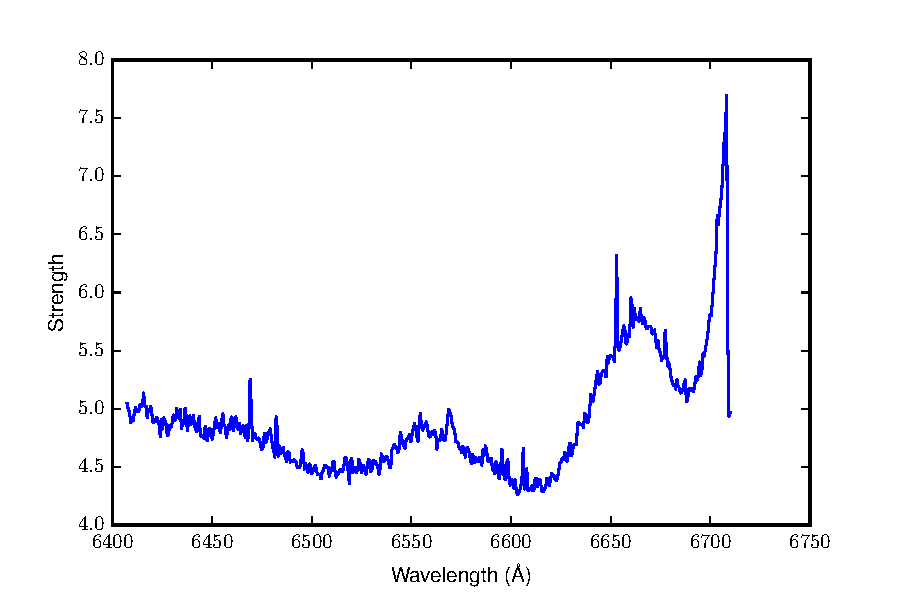
\includegraphics[width=\linewidth]{1h-l115u120-spectrum.pdf}
\captionof{figure}{Pixel 115 to Pixel 120. Peak wavelength: 6568.7 $\Omega$, Redshift: 270 km/sec}
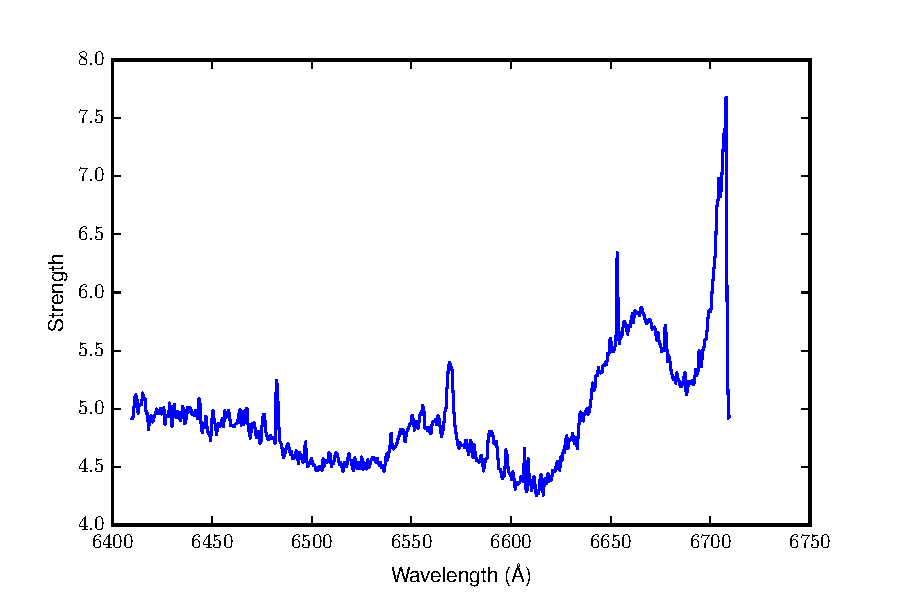
\includegraphics[width=\linewidth]{1h-l120u125-spectrum.pdf}
\captionof{figure}{Pixel 120 to Pixel 125. Peak wavelength 6569.1 $\Omega$, Redshift: 291 km/sec }
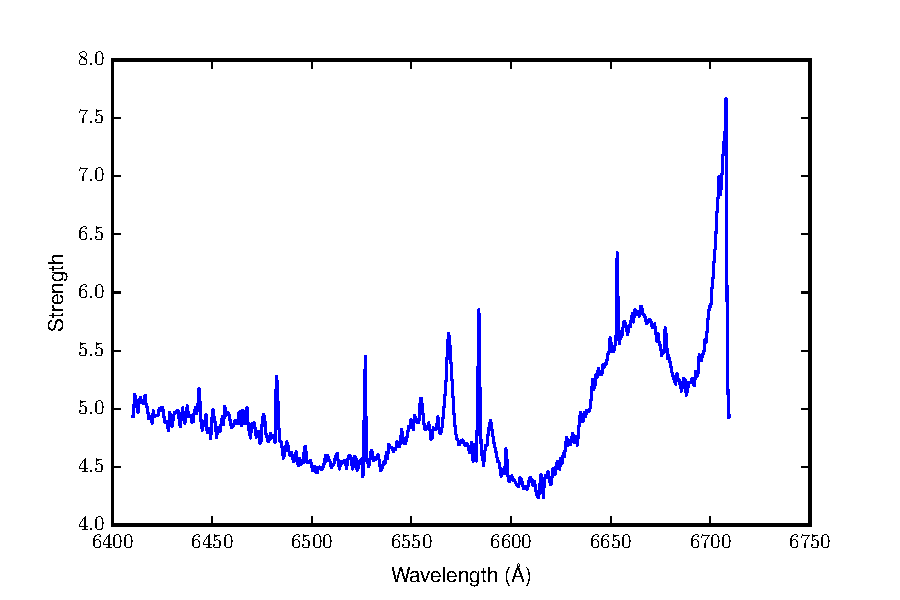
\includegraphics[width=\linewidth]{1h-l125u130-spectrum.pdf}
\captionof{figure}{Pixel 125 to Pixel 130. Peak: 6583.9 $\Omega$, Redshift: 962 km/sec. Very odd spikes have arisen in the data, and the Gaussian most likely fit the wrong peak.}
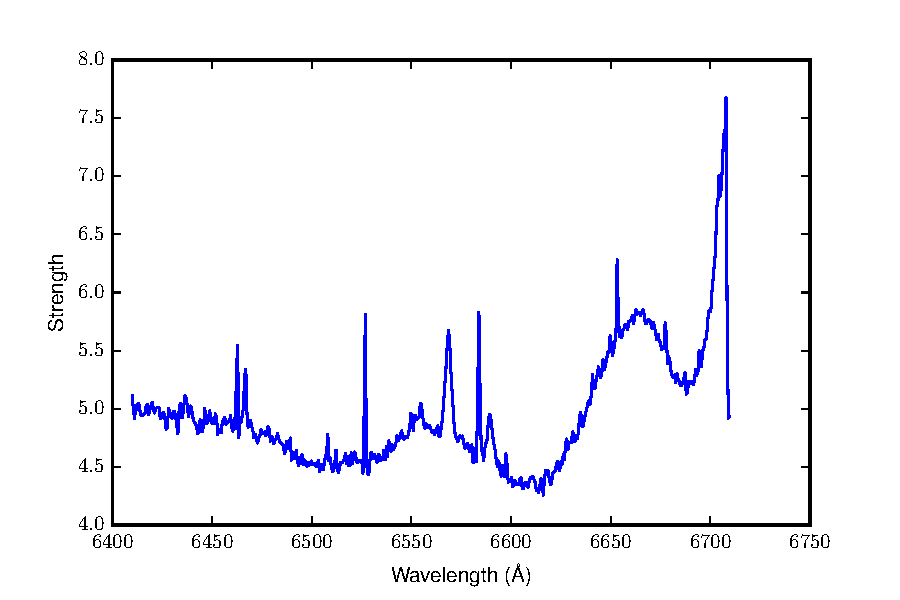
\includegraphics[width=\linewidth]{1h-l130u135-spectrum.pdf}
\captionof{figure}{Pixel 130 to Pixel 135. Peak: 6583.9 $\Omega$, Redshift: 962 km/sec. Again this redshift is too high.}
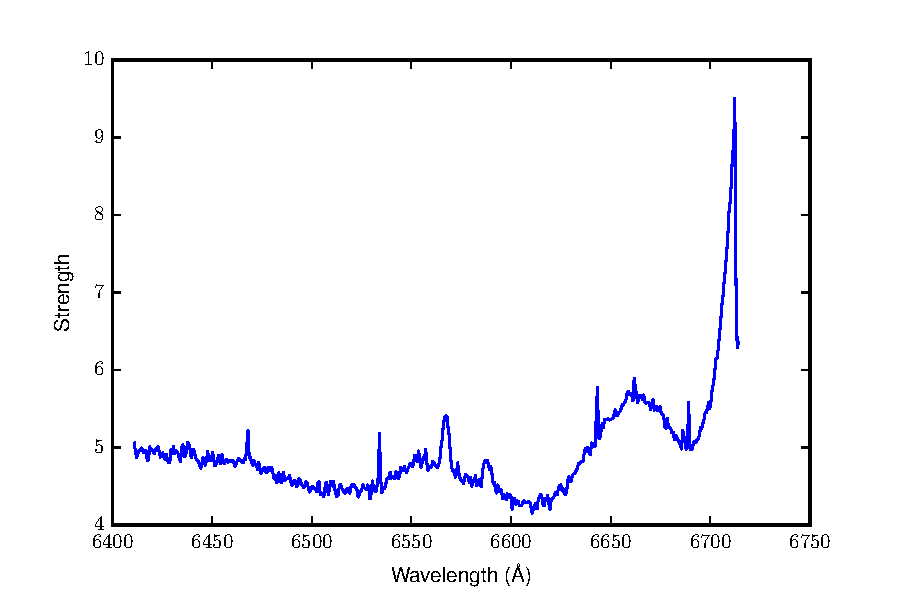
\includegraphics[width=\linewidth]{1h-l135u140-spectrum.pdf}
\captionof{figure}{Pixel 135 to Pixel 140. Peak: 6567.2 $\Omega$, Redshift: 203 km/sec }
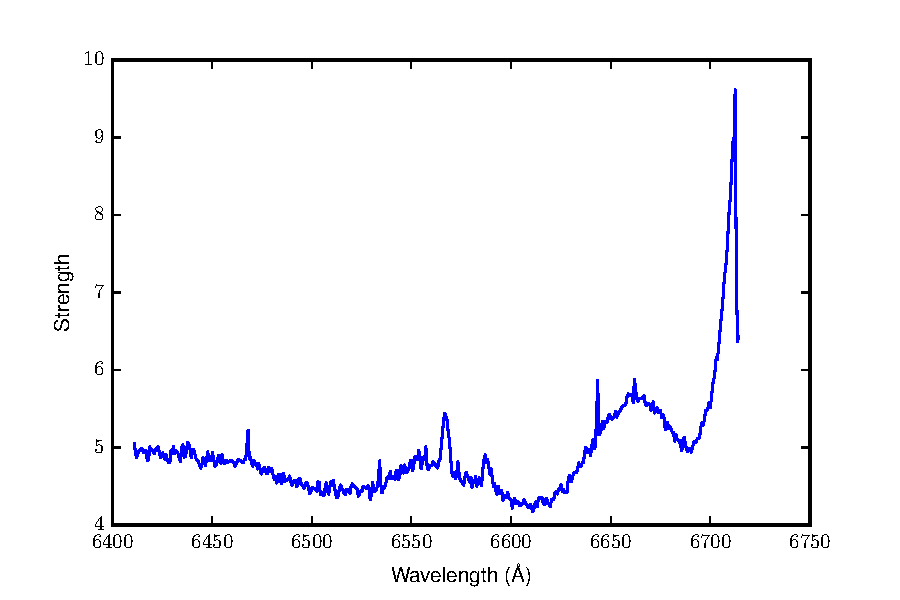
\includegraphics[width=\linewidth]{1h-l140u145-spectrum.pdf}
\captionof{figure}{Pixel 140 to Pixel 145. Peak: 6566.7 $\Omega$, Redshift: 180 km/sec}
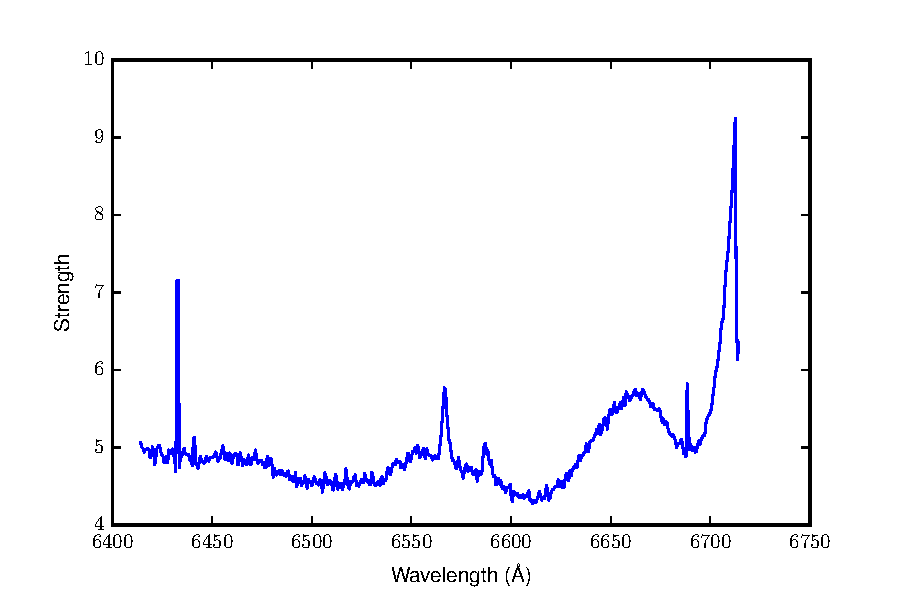
\includegraphics[width=\linewidth]{1h-l145u150-spectrum.pdf}
\captionof{figure}{Pixel 145 to Pixel 150. Peak: 6566.5 $\Omega$, Redshift: 171 km/sec}
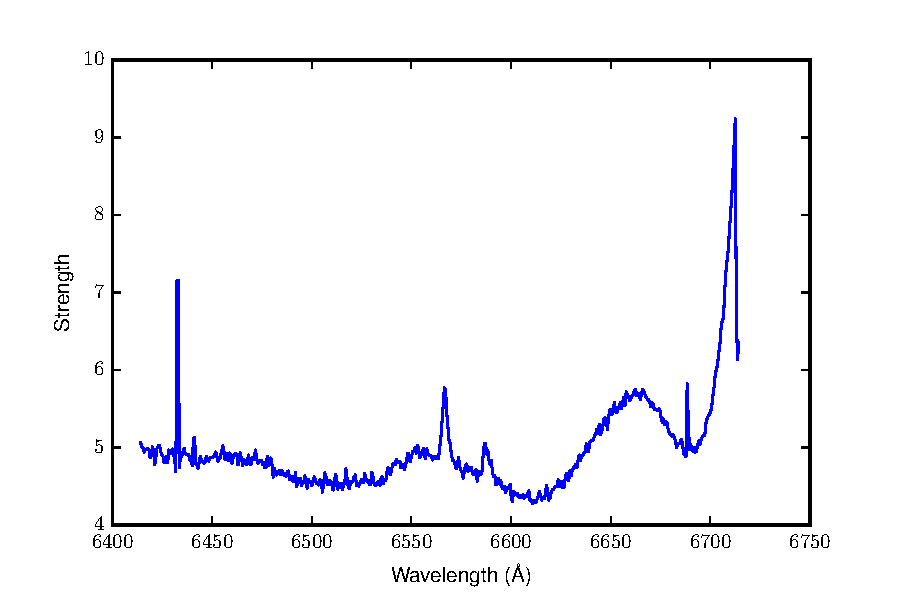
\includegraphics[width=\linewidth]{1h-l150u155-spectrum.pdf}
\captionof{figure}{Pixel 150 to Pixel 155. Peak: 6566.5 $\Omega$, Redshift: 171 km/sec}
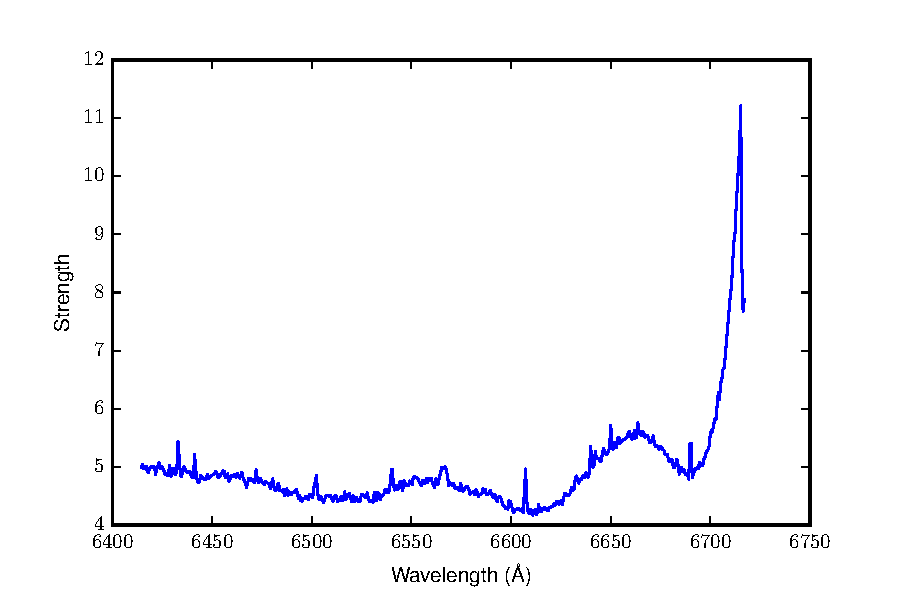
\includegraphics[width=\linewidth]{1h-l155u160-spectrum.pdf}
\captionof{figure}{Pixel 155 to Pixel 160. Peak: 6566.9 $\Omega$, Redshift: 190 km/sec}
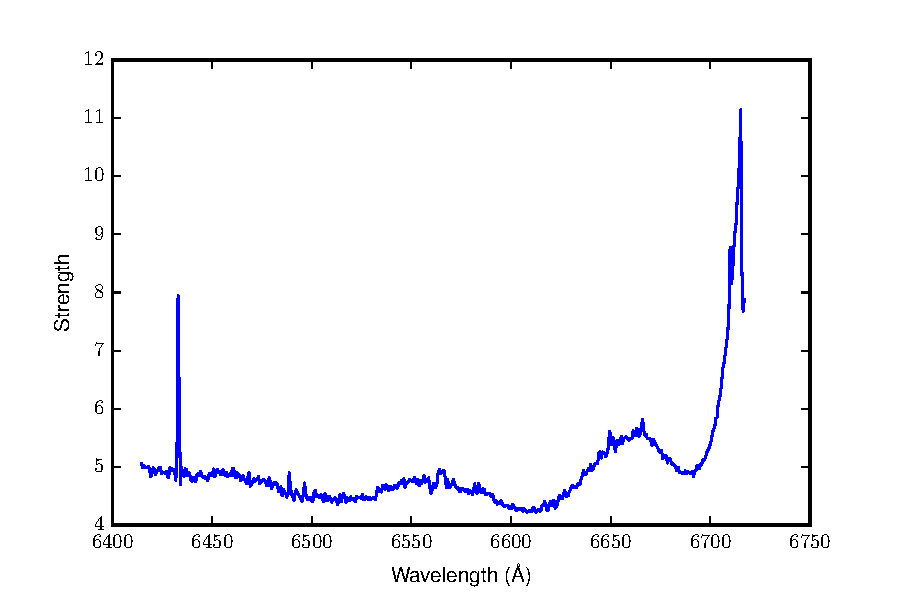
\includegraphics[width=\linewidth]{1h-l160u165-spectrum.pdf}
\captionof{figure}{Pixel 160 to Pixel 175. Peak: 6564.0 $\Omega$, Redshift: 54 km/sec}

While there seemed to be a genuine trend for a rotation curve in the data set, the two massive outliers from pixels 125 to 135 pixels indicate that the data is unreliable. The 60 minute observation was also marked with more observational issues than the 120 minute observation. We had less confidence in controlling drift and managing the dome in this observation session. The 120 minute observation was relatively smooth.

\subsection*{120 Minute Exposure}

The 120 minute exposures were taken on May 27th. The following graphs are scaled to the vicinity of H$\alpha$, at 6563 $\Omega$, with a range of 50 $\Omega$.

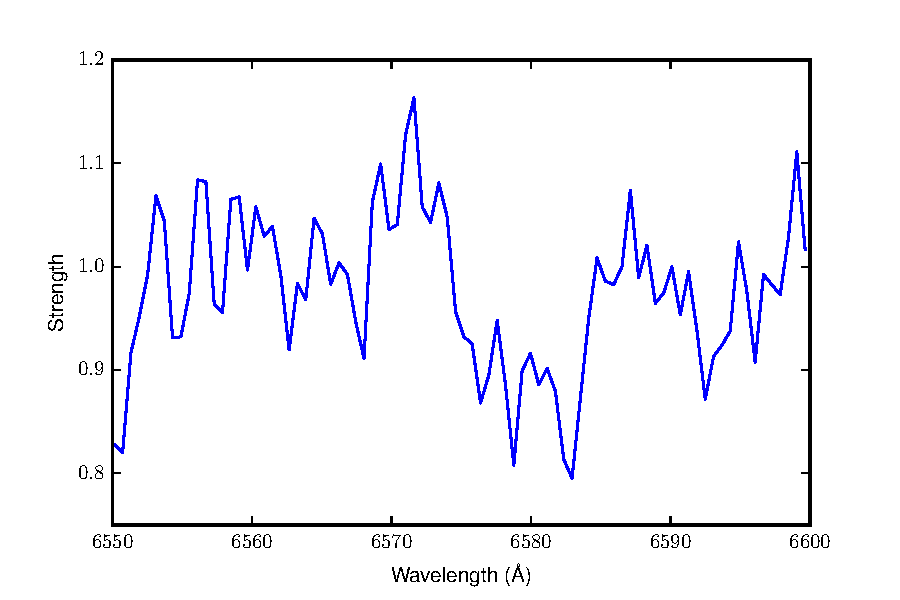
\includegraphics[width=\linewidth]{M82-l115u120-spectrum-6550-to-6600.pdf}
\captionof{figure}{Pixel 115 to Pixel 120. The H$\alpha$ peak appears fuzzy. Peak wavelength: 6571.6 $\Omega$, Redshift: 402 km/sec}
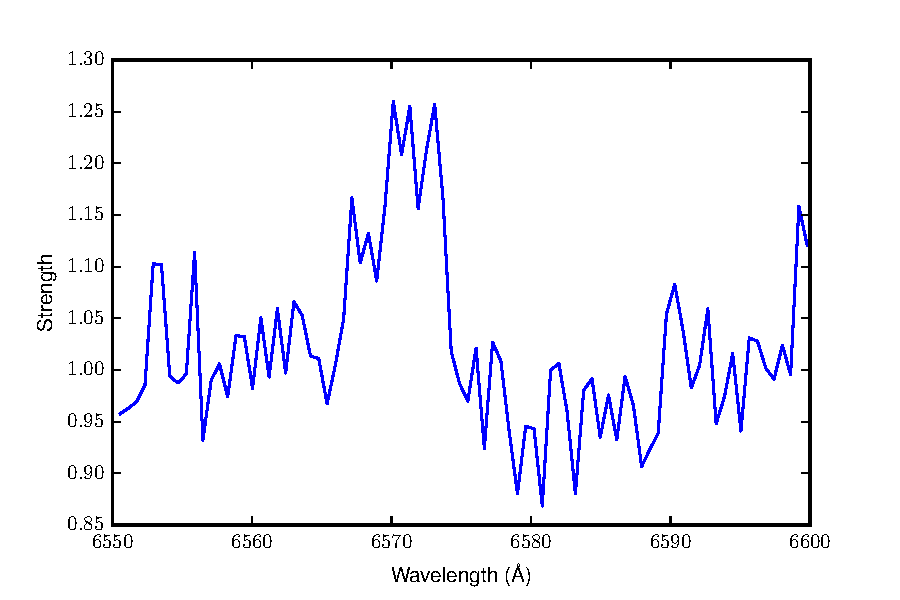
\includegraphics[width=\linewidth]{M82-l120u125-spectrum-6550-to-6600.pdf}
\captionof{figure}{120-125. Peak: 6570.1 $\Omega$, Redshift: 335 km/sec}
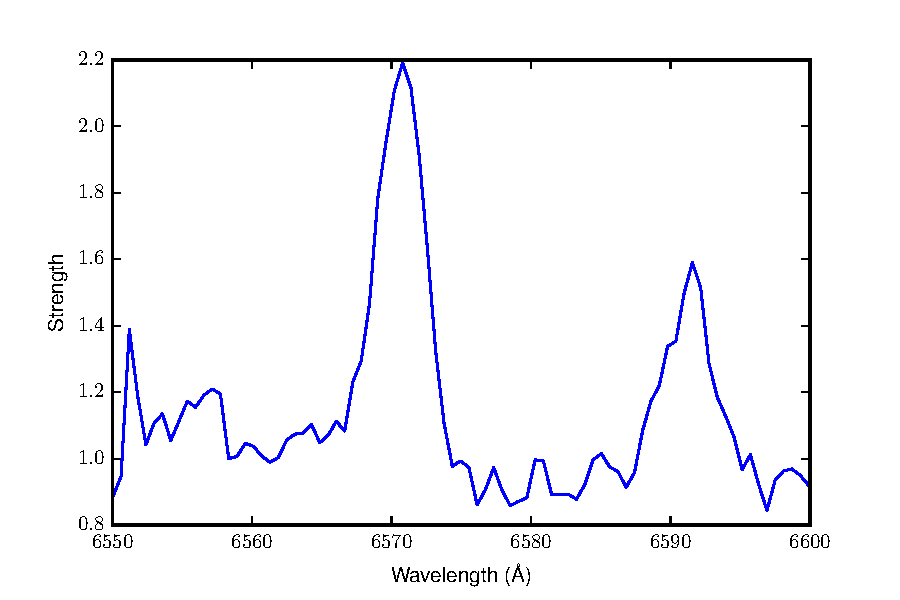
\includegraphics[width=\linewidth]{M82-l125u130-spectrum-6550-to-6600.pdf}
\captionof{figure}{125-130. The H$\alpha$ peak appears clearer. Also, an ionized Nitrogen line can be seen. Peak: 6570.8 $\Omega$, Redshift: 365 km/sec}
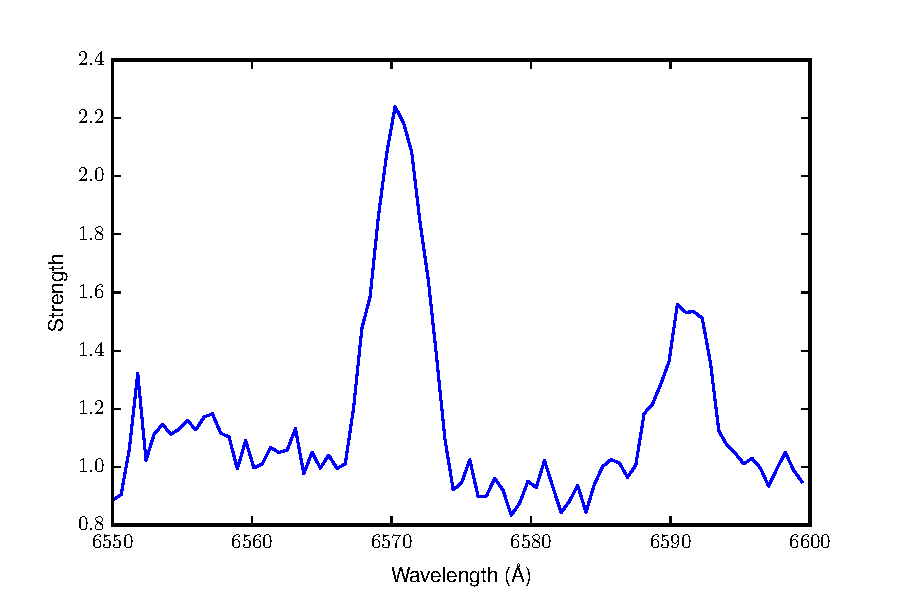
\includegraphics[width=\linewidth]{M82-l130u135-spectrum-6550-to-6600.pdf}
\captionof{figure}{130-135. Peak: 6570.3 $\Omega$, Redshift: 341 km/sec }
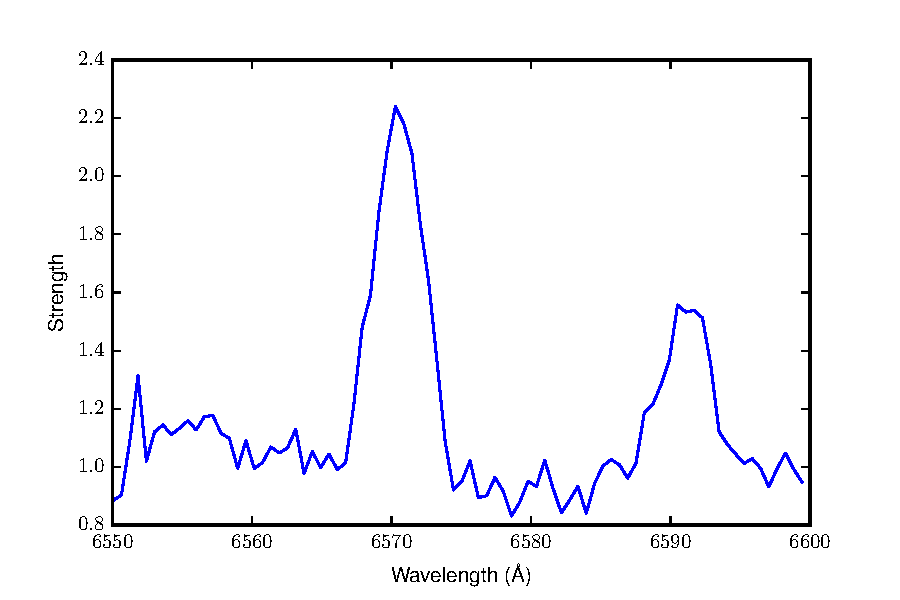
\includegraphics[width=\linewidth]{M82-l135u140-spectrum-6550-to-6600.pdf}
\captionof{figure}{135-140. Peak: 6570.3 $\Omega$, Redshift: 341 km/sec}
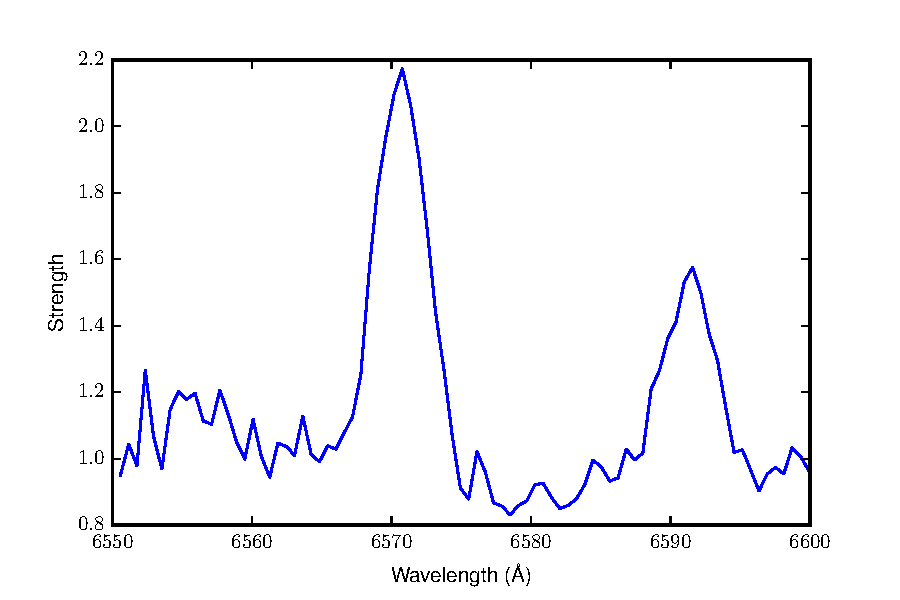
\includegraphics[width=\linewidth]{M82-l140u145-spectrum-6550-to-6600.pdf}
\captionof{figure}{140-145. Peak: 6570.8 $\Omega$, Redshift: 364 km/sec. The redshift pattern is distinct; the peak continues to move to shorter wavelengths.}
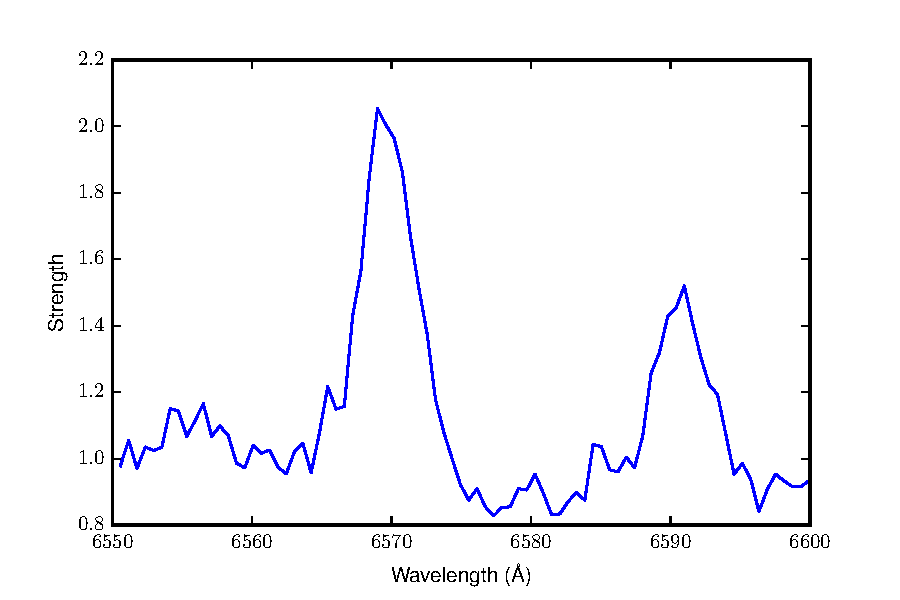
\includegraphics[width=\linewidth]{M82-l145u150-spectrum-6550-to-6600.pdf}
\captionof{figure}{145-150. Peak: 6569.0 $\Omega$, Redshift: 283 km/sec}
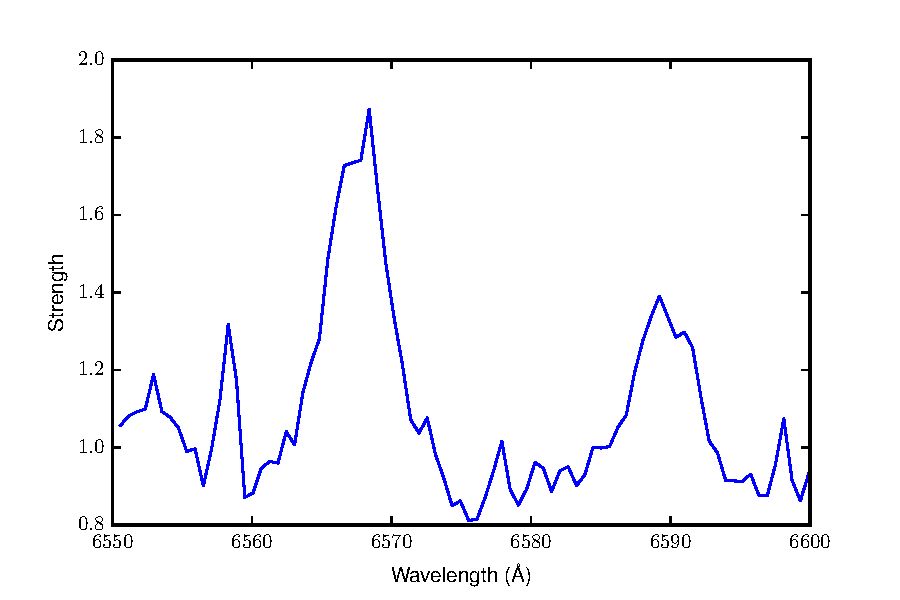
\includegraphics[width=\linewidth]{M82-l150u155-spectrum-6550-to-6600.pdf}
\captionof{figure}{150-155. Peak: 6568.4 $\Omega$, Redshift: 256 km/sec}
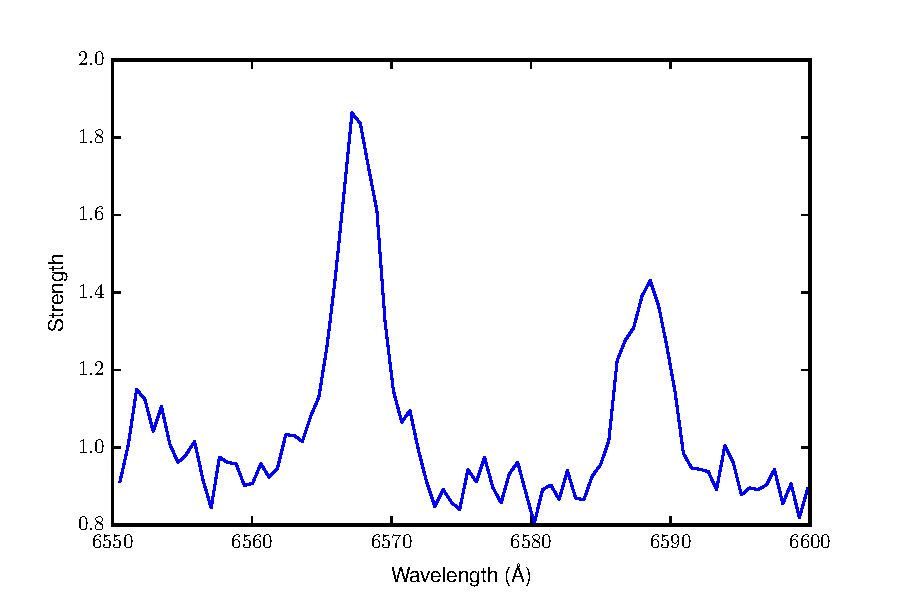
\includegraphics[width=\linewidth]{M82-l155u160-spectrum-6550-to-6600.pdf}
\captionof{figure}{155-160. Peak: 6567.2 $\Omega$, Redshift: 199.5 km/sec}
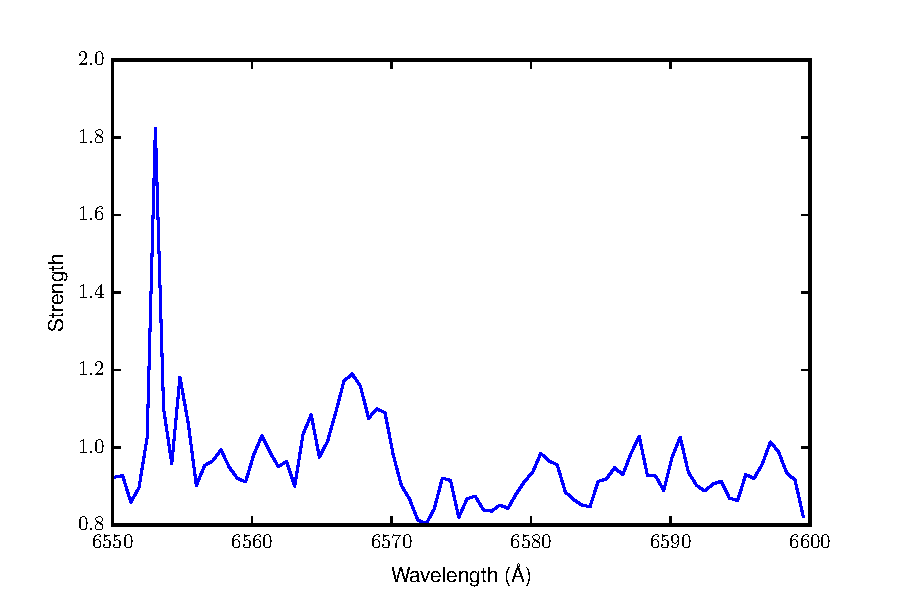
\includegraphics[width=\linewidth]{M82-l160u165-spectrum-6550-to-6600.pdf}
\captionof{figure}{160-165. The pattern breaks up, and the peak disappears. Peak 6553.1 $\Omega$, Redshift: -444 km/sec}
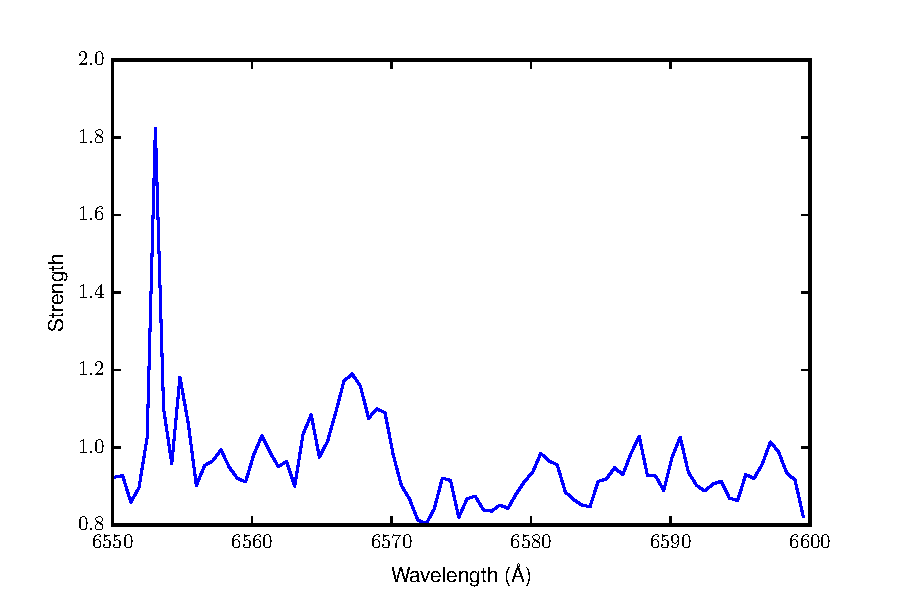
\includegraphics[width=\linewidth]{M82-l165u170-spectrum-6550-to-6600.pdf}
\captionof{figure}{165-170. 6553.2 $\Omega$, Redshift: -450 km/sec }
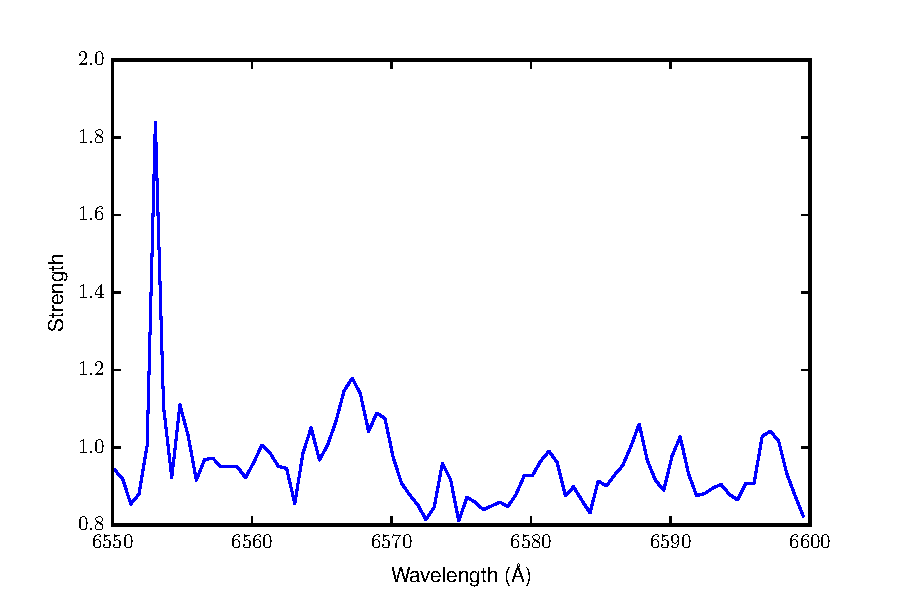
\includegraphics[width=\linewidth]{M82-l170u175-spectrum-6550-to-6600.pdf}
\captionof{figure}{170-175. 6553.3 $\Omega$, Redshift: -456 km/sec}
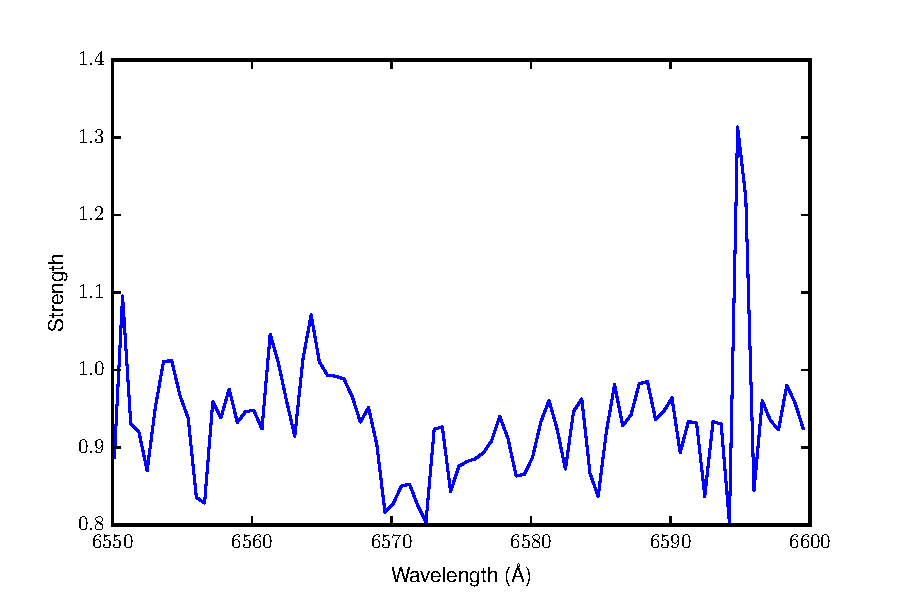
\includegraphics[width=\linewidth]{M82-l175u180-spectrum-6550-to-6600.pdf}
\captionof{figure}{175-180. 6594.8 $\Omega$, Redshift: 1460 km/sec}


The general trend of radial-distance correlation with orbital velocity is confirmed by this graph. We can see that in traversing as little as 5 pixels (3.5 arcminutes), velocity decreases by up to 80 km/sec. This agrees with experimental data on M82's rotation curve: at the point of steepest dropoff, the orbital velocity drops 150 km/s in 4kpc, about 4' considering M82's actual and apparent diameter (\cite{rotation}). The similarity between these two values confirms the integrity of our measurements.

However the last 4 datasets,  demonstrate more dramatic dropoffs. These data points are suspicious; qualitatively H$\alpha$ seems to disappear from the spectrum entirely by pixel 160. The Gaussian fit in this situation is then invalid since there is no H$\alpha$ line. The absence of H$\alpha$ is most likely due to the lack of starburst regions outside the center of M82. If outer points of the galaxy do not have robust H II regions, our measurement technique at these points is compromised.

A concern in this analysis is the location of the radial center. Redshifts on either sides of the radial center should have a differential of about 400 km/sec (M82's orbital velocity is 200 km/sec peak to peak). We don't see this feature in our data, which is problematic. This is most likely due to telescope drift errors. 


\section*{Conclusions}

Extensive research on the rotation curve of M82 has been completed before. Papers indicate the exceptional behavior of the rotation curve: there is a prototypical steep nuclear rise, but a sharp dropoff follows it, obeying Keplerian law (\cite{rotation}). This behavior is theorized to be a consequence of interaction with nearby galaxy M81. A close encounter between the two galaxies may have caused a strong tidal truncation of the disk (\cite{encounter}). Our own spectroscopy measurements replicated this steep Keplerian dropoff.

There is no consensus in the literature on the nature of M82's rotation curve at outer radii, however. The verified measurement of the rotation curve completed in 1998 hinged on H I radiation outside of 1 kpc from the radius -- this radiation is likely disrupted and not solely from rotation. It is hypothesized that the H I signature is characterized by tidally induced, non-rotational components, thus compromising the integrity of the data (\cite{peculiar}). Our method of using H$\alpha$ emission lines did not shed any more light on outer radii than previous experiments. Our barrier was the lack of starburst activity outside of the center of M82.

The mass distribution of M82 is also inconclusive, though some aspects are well-accounted for. M82's mass has a much larger contribution from atomic and molecular gas than other spiral galaxies. The high gas content obscures mass estimation and dust attenuation; unpredictable tidal motions make the endeavor challenging and uncertain (\cite{measure}). Dust and other artifacts may have been obstacles in our measurement; however, it is unlikely that these small perturbations had any impact on our final results.


{\centering 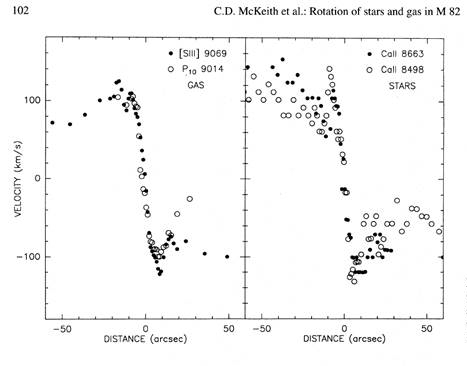
\includegraphics[width=228pt]{rotationcurve.jpg}\par}
\captionof{figure}{The experimentally verified rotation curve for M82. Note that data still does not exist at larger radial distances -- those regions are more difficult to pinpoint even with more precise methods}

We produced an approximation of Keplerian dropoff in M82, proving that studying the starburst galaxy through the Stanford Student Observatory is feasible. With further refinement to the experiment, such as minimizing unknown error propagation, more elaborate, rigorous rotation curves can be obtained.


\bibliographystyle{ksfh_nat}

\bibliography{references}













\label{lastpage}

\end{document}